\section{Introduction} \label{sec:intro}
% Introduction
In 2017, the European Union counted around $25300$ fatalities on the EU roads, of which 46\% were vulnerable road users. Although the EU roads account for the safest roads in the world, the number of road fatalities have stagnated in the past few years. At this rate, the EU's goal of reaching fewer than $16000$ fatalities in 2020 could not be achieved. Especially vulnerable road user fatalities have not decreased at the same pace as the overall population. Any progress to increase the safety of vulnerable road users will have a significant impact to the road fatality rate. \cite{vademecumeu2018road} \\

\glspl{AV} are expected to increase road safety because the autonomy would erase the effects of human error \cite{cui2019review}, since more than 90\% of the accidents is caused by human error \cite{eu2020website}.

% Implement new Introduction Around here
However, \glspl{AV} are not yet safe enough to deploy on the roads and still a lot of research should be done before fully autonomous vehicles can be introduced to the market \cite{okuda2014survey} \cite{cui2019review}. \\

One of the current challenges to autonomous driving is to capture road user intent and to make accurate real-time trajectory predictions of other road users \cite{ohn2016looking}. Especially predicting the behavior of \glspl{VRU} is important \cite{ohn2016looking} \cite{cara2015classification} because good anticipation of a \gls{VRU}'s behaviour results in faster reactions and thus can prevent more accidents \cite{djuric2020uncertainty}. Predicting \gls{VRU} behavior is additionally challenging compared to predicting other (motorized) road users, because "\gls{VRU} motion follows complex patterns constrained by static and dynamic obstacles along the path." \cite{chou2020predicting} \\

This literature study gives an overview of what the current research areas and challenges for the future are regarding motion prediction of vulnerable road users. Based on this literature study I will write a research proposal for my Master thesis. \\

This chapter describes the problem of motion prediction and elaborates on current solutions and their limitations. Then, one main research question and five sub-questions are asked to investigate the stated problem. This chapter ends with a short overview of the content of each chapter.

\subsection{Problem Description} 
%Problem
The problem of motion prediction is an inferencing task. Based on evidence in the form of current and/or past observations and obtainable experience, future states (trajectories) of one or more actors must be predicted for a pre-determined time horizon, within a certain accuracy and certainty, which needs to be executed within a specific time limit. This problem statement will be explained more elaborately in these following paragraphs. \\

Actors, in this problem statement, are traffic participants including, but not limited to, cars, riders, cyclists and pedestrians (\glspl{VRU}). \\

The evidence that supports the actor's predictions can have the form of current and/or past observations, and obtainable experience. The current and past observations are sensor data acquired from the environment (observations) by either static observers (the sensors are static and record the environment) or dynamic observers (the sensors move within the environment while recording it) or both.
Then, obtainable experience are generalizations of traffic, including traffic behavior and traffic environments (experience). These generalizations can be based on statistics, they can be based on assumptions, and they can be learned using historic observations. \\

Based on the investigated literature, the future states can be represented as one of the three following forms in the predictions. 

\begin{enumerate}
	\item The predictions are estimated future state values of an actor's centroid, including its coordinates and sometimes orientations, which are projected into the environment representation.
	\item The predictions are estimations of the future actor's representation within the current environment representation.
	\item The predictions are estimations of the entire future environment representation.
\end{enumerate}

\begin{figure}[h!]
	\centering
	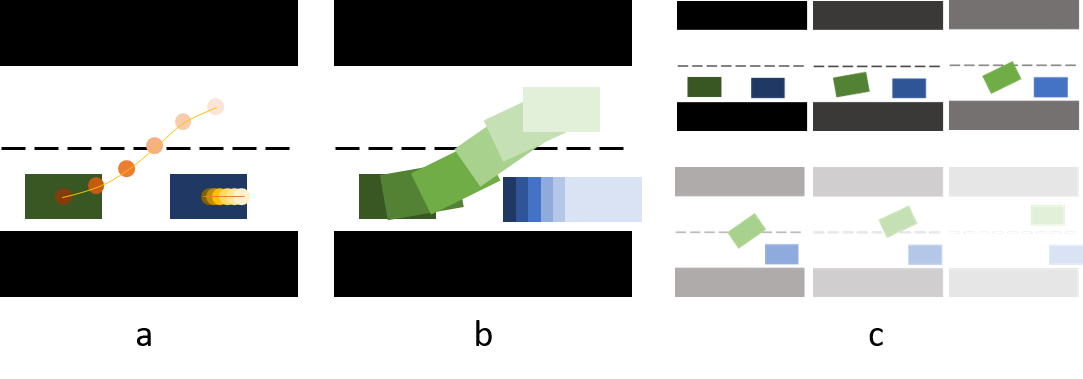
\includegraphics[width=0.8\linewidth]{Figures/Introduction/Prediction_forms}
	\caption{This image shows the three prediction forms encountered in the literature. The black and white parts represent a road. The green and blue squares are representations of vehicles. The predictions are shown using a more fading color the further the prediction goes into the future. Figure a shows the prediction of future centroids projected into the environment representation. Figure b shows the prediction of future actor representations within the environment (the complete vehicles are predicted instead of the centroids only). Figure c shows the prediction of the entire future environment. In this case, also a prediction of the environment (road) is provided.}  
	\label{fig:pred_froms}
\end{figure}

Finally, the problem statement mentions a time horizon, that the predictions must be within a certain accuracy and certainty, and that it needs to be executed within a specific time limit. The time horizon is the amount of time into the future that the prediction must span. Ideally, the time horizon, the accuracy, the certainty, and the execution time of the predictions should be infinitely, exact, complete, and instantaneously respectively. However, this is not possible in practice. Therefore, I think a suitable prediction method should perform further into the future, more accurate, with more certainty, and faster than a human can perform the task. Within the context of \glspl{AV}, this is a reasonable requirement in order for the \gls{AV} to be able to perform safer than humans can.   


\subsection{Current Solutions}

Table \ref{tab:overview_mot_pred} in Appendix \ref{app:appendixA} shows an overview of recent motion prediction papers and their respective methods. It is notable that most methods use a form of deep learning to predict trajectories in any of the forms as described in the problem description. What is also striking, is that relatively few papers have performed research which includes \glspl{VRU} in which the observer is dynamic (from a vehicle's point of view). Still, it is important that \gls{VRU} behavior prediction is investigated. \gls{VRU} collisions are likely to be fatal which makes accurate and early motion prediction necessary in order to respond safely to their actions \cite{rehder2018pedestrian}, \cite{chou2020predicting}, \cite{uah2020d4}. Therefore, \gls{VRU} behaviour prediction is a relevant research topic regarding \glspl{AV}.\\
A major challenge in this research area is to predict \gls{VRU} motion for the long term. However, research on this topic faces a multitude of challenges. Accurate long-term predictions require the incorporation of environmental and social context. Moreover, implementing uncertainty and multimodality of the predictions and making the predictions fast enough for real-time applications in \glspl{AV} are also challenges that need to be solved. These major challenges and recent research to find solutions are described in the following subsections. 

\subsubsection{Long-term motion prediction}
For motion prediction, a prediction for which the prediction time horizon is more than 2 seconds is considered long-term \cite{hormann2020long}. Compared to other road users, \glspl{VRU} are highly maneuverable which makes it challenging to predict their behavior, especially for the long-term \cite{xiong2019recurrent}, \cite{rehder2018pedestrian}, \cite{rehder2018pedestrian}. Most prediction models assume that \gls{VRU} behavior is intention-driven and that those intentions can be inferred from certain cues, other than dynamics \cite{rehder2018pedestrian}. Therefore, detecting cues related to \gls{VRU} behavioral changes is important for achieving accurate long-term predictions \cite{pool2017using}. These cues can be related to the \gls{VRU}'s environment (e.g. traffic lights, zebra's, obstacles) or to the \gls{VRU}'s social interactions (e.g. evasion of other \gls{VRU}'s, distancing due to social norms, nearing another \gls{VRU}). The following two paragraphs elaborate on the incorporation of environmental and, respectively, social context in prediction models. Besides using cues to predict \gls{VRU}'s behavior, implementing the uncertainty of the predictions and incorporating multimodality is also researched, as well as making the models fast enough so that they can be implemented real-time on \glspl{AV}. These topics are also discussed below. 

\subsubsection{Environmental context}
Environmental context consists of the static and dynamic obstacles and semantic meaning within an actor's surroundings.
Research suggested to incorporate environmental context because an actor's trajectory is highly influenced by its environment. Scene context can constrain the actor in its planned motions \cite{chou2020predicting}, \cite{pfeiffer2018data}, \cite{sadeghian2019sophie}, \cite{manh2018scene}. Especially to anticipate critical situations, taking into account the environmental context is expected to increase the prediction accuracy \cite{uah2020d4}. The challenge is how to model that environmental context so that it is semantically representative, highly discriminative and generalizable to a variety of complex scenes so that it can be used as evidence to enable inferences about an actor's future trajectory \cite{varshneya2017human}.

\cite{pool2017using} Shows that leveraging prior knowledge about an actor's environment can improve the trajectory predictions. Therefore, they suggest to extend the incorporation of environmental context even more with the expectation that it will further increase the prediction accuracy.  


\subsubsection{Social Context}
Social context consists of the static and dynamic actors, their semantic meaning, and their interactions within an actor's surroundings.
When an actor navigates, it constantly tries to anticipate movements of surrounding actors to envision more than one feasible path it could take in order to adjust its own path and maneuver past or aside those surrounding actors \cite{sadeghian2019sophie}, \cite{manh2018scene}. Therefore, one of the main factors that influence an actor's behavior is the its social context. It is expected that by incorporating social context into prediction models, the accuracy will increase significantly \cite{pfeiffer2018data}. 

Especially for pedestrian behavior, the social and environmental context is expected to be the leading evidence for predicting their behavior because pedestrians "are not expected to use any active forms of communication when interacting with vehicles and other road users" \cite{uah2020d4}. 


\subsubsection{Uncertainty and Multi-modality}
For the safety of AVs, uncertainty estimations for predictions are critical \cite{djuric2020uncertainty}. If an AV is aware of the confidence of its predictions, it can adjust its planned course to minimize the risk of collisions \cite{huang2019uncertainty}. For example, if an AV predicts that a pedestrian will not cross the road, but the confidence of that prediction is very low, the AV can adjust its course by leaving more room for the pedestrian in case the prediction is false. Without knowing the confidence of a prediction, such risk-avoiding course adjustments cannot be made. Besides including uncertainty estimations, it is important that predictions are multimodal. VRU behaviour is inherently multimodal because they easily change their course which is highly dependent on their environment \cite{cui2019multimodal}, \cite{tang2019multiple}. Incorporating multimodality is a challenge, because it requires good probability estimations and knowledge of the different modes. It either requires explicit labeling of the modes prior to training \cite{tang2019multiple}, or the modes could be learned. Because probability estimations are needed to make multimodal predictions, these methods are often researched together. \\
\cite{keller2013will} compares four different multimodal prediction models related to Bayesian principles. These models return the probability of stopping (whether a nearing pedestrian will stop, instead of cross the road). However, only two motion modes are considered in this research. \cite{pool2017using} Uses a Mixture of Linear Dynamical Systems to predict the probabilities of a cyclists going in one of the five pre-determined direction modes. This model also takes into account information about the road topology to enhance the predictions. The downside of these Bayesian models is that the computation time increases when more modes are added and when more context information is incorporated in the predictions. Moreover, adding more modes is a challenges in complex environments in which it is unclear what directions an actor can go to. Therefore, deep learning models are devised that can include multimodality in the predictions by learning the modes in a latent space and incorporating learned features of the VRU's context. \\
\cite{rehder2018pedestrian}, \cite{cui2019multimodal}, \cite{brito2020social} investigated deep learning models that, respectively, predict multimodal trajectories by training a network to learn the parameters of a Mixture Density Network that predicts multiple trajectories, train a network to choose the best of M hypothetical trajectory modes, and train a variational RNN that learns a conditional distribution of available modes from which the output Gaussian Mixture Model can be sampled. Although these methods all provide probabilities for the different available trajectory modes, still they do not provide a confidence estimation the model has about the multimodal predictions. \cite{huang2019uncertainty}'s research adds a confidence estimator to their multimodal prediction method that estimates the confidence of multiple predictors. The predictor with the highest confidence value is considered for the trajectory prediction. 

\subsubsection{Real-time motion prediction}
Fast real-time computation is important in order to implement the prediction model on AVs. 
\cite{djuric2020uncertainty} Addresses the importance of real-time execution of prediction models. They state that certain prediction methods (e.g. Bayesian Networks and Inverse Reinforcement Learning) are inefficient and thus not feasible for real-time applications such as AVs. Therefore, it is important that the prediction methods are efficient enough so they can be applied online in AVs to increase VRU safety. Their method of using a CNN to predict future trajectories was succesfully tested real-time in an AV. However, this method only predicts future trajectories of vehicles, not VRUs. \\
\cite{brito2020social} stresses the importance for real-time predictions for applications in AVs as well. They developed the Social-VRNN that takes samples from a variational RNN's conditional distribution to predict pedestrian trajectories. Previous research used other methods, such as Generative Adversarial Networks (GANs), which required more samples for accurate predictions compared to the Social-VRNN, making the Social-VRNN much faster. However, this method does not yet perform in real-time.  \\
\cite{chou2020predicting} aims for the most efficient motion prediction models without it affecting the accuracy because it "is necessary to achieve real-time inference onboard an SDV in crowded urban environments comprising large number of VRUs" \cite{chou2020predicting}. Without real-time online motion prediction, AVs cannot make use of these methods and the safety of VRUs will not improve. They developed a real-time motion prediction method, using a CNN, for all road users. Their solution shows promising results, but the dataset requires more VRU data to match the state-of-the-art prediction accuracy. 

\subsection{Research Questions}
State-of-the-art research shows that Deep Learning methods provide means to include environmental and social context, as well as uncertainty information, to make better, long-term, path predictions including those of \glspl{VRU}. Several Deep Learning methods use \glspl{OGM}, a grid-based representation of the environment obtained from sensors on \glspl{AV}, as input data to predict future \glspl{OGM} for the long-term. \glspl{OGM} contain occupancy data of the \gls{AV}'s environment which is often extended with uncertainty information of the occupied areas. Furthermore, the \gls{OGM} can be extended with additional information layers such as semantics and dynamics of the occupied regions. Correlations of the environment and its actors can be captured when the \gls{OGM} is processed by a Deep Learning network. Predicting \glspl{OGM} is expected to be more accurate, also for long-term predictions, due to the amount of information that can be stored in the OGM. Attempts to make real-time \gls{OGM} predictions are succeeding (Mohajerin \cite{mohajerin2019multi} shows that it can take 60ms to predict \glspl{OGM} 1s into the future), making this environment representation method a promising one for state prediction research. \\
 
Because of the potential of \glspl{OGM}, this literature review focuses on the prediction of \glspl{OGM} using Deep Learning. The following main research question is asked: \textit{"What are currently the best methods to perform \gls{OGM} prediction?"} 
This question will answered using the answers of the following sub-questions:

\begin{enumerate}
	\item What OGM form is most suitable to use in OGM prediction methods?
	\item What dataset is most suitable to generate OGM sequences for OGM prediction?
	\item What is the best metric to determine the quantitative accuracy of a predicted OGM?
	\item What Deep Learning network is best to use for OGM prediction?
	\item What method generates the best OGM predictions?
\end{enumerate}


\subsection{Chapter overview}
The posed research questions will be answered in the following chapters of this literature review. Chapter \ref{sec:ogm} provides information about \glspl{OGM} and answers the first research question. In chapter \ref{sec:datasets}, criteria are set which an ideal dataset should meet to use it for \gls{OGM} prediction. This chapter will answer the second research question. The third research question will be answered in chapter \ref{sec:metrics}, in which several metrics to determine the quality of \glspl{OGM} are compared and tested against some criteria that are required for accurate error estimations of \gls{OGM} predictions. Chapter \ref{sec:seqDLnets} provides an overview of deep learning networks that process sequential data for prediction purposes. In this chapter, the answer to the fourth research question is provided. The last research question will be answered in chapter \ref{sec:ogm_methods}, in which several methods are highlighted that use \glspl{OGM} for their state predictions. Chapter \ref{sec:conclusion} contains a conclusion in which the main research question of this literature review is answered. The final chapter is a research proposal for my Master thesis to which the conclusion of this literature review provides the basis.




%% After the Challenges: Each challenge becomes a topic/section
%% Long term motion prediction: discuss most used methods up until deep learning methods
%% Discuss how later the incorporation of environment, social, uncertainty/mutlimodality was also incorporated
%% And what methods are used for that
%% Dicuss Why real-time motion prediction is important and what the fastest computation times are for each other challenge
%% And how faster methods can be researched 
%%

%%% NEW LIT PART

%% Before, the main challenges to motion prediction are described. Then, ... thought of using OGMs to predict the future because in an OGM env and social context can be incorporated, multimodal paths and uncertainty can be computed, and some prediction methods can even perform real-time. But what are the advantages and disadvantages? Is it really better?



